\documentclass[tikz]{standalone}
\usetikzlibrary{calc, intersections, math}

\begin{document}
	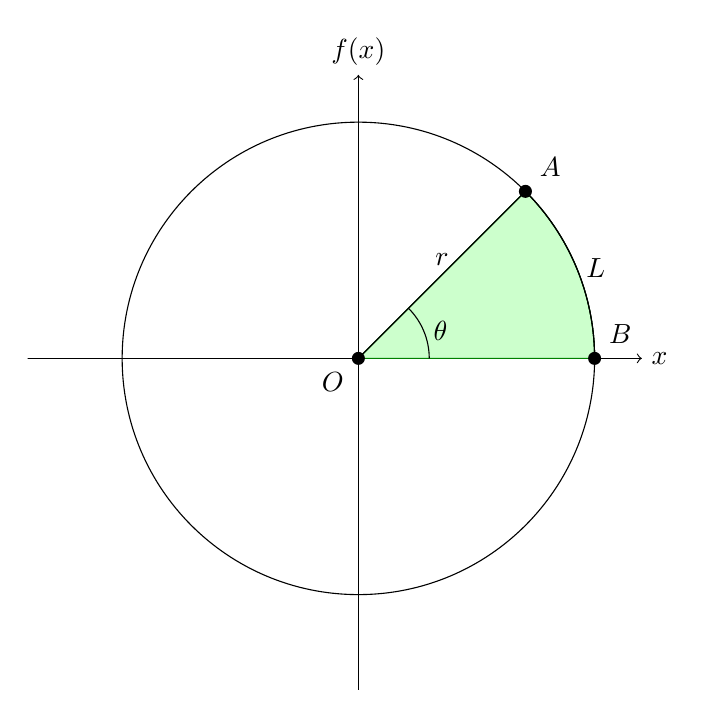
\begin{tikzpicture}[scale=3, mystyle/.style={circle,fill,scale=0.5}]

		% Set the angle of the central arc
		\tikzmath{\angle = 45;}

        % selecting the first quadrant
        \clip (-1.4,-1.4) rectangle (1.4,1.4);
        % setting up the Cartesian Grid. Note "help lines" = "gray, very thin"
        %\draw[step=.2cm,help lines] (-1.5,-1.5) grid (1.5,1.5);
        % setting up the real and imaginary axis. 
        \draw[->] (-1.5,0) -- (1.2,0) coordinate (x axis) node[right] {$x$};
        \draw[->] (0,-1.5) -- (0,1.2) coordinate (y axis) node[above] {$f(x)$};
		% draw and fill the circular segment
		\filldraw[fill=green!20!white, draw=green!50!black] (0,0) -- (1cm,0)  arc  (0:\angle:1cm) -- cycle;
		% add the unti circle
		\draw (0,0) circle (1cm);
		% draw and label the central arc AOB
		\draw 
			(0,0) 
				node[mystyle, label=below left:{$O$}] (O) {} -- 
				node[above] {$r$}
			(\angle:1cm) 
				node[mystyle, label=above right:{$A$}] (A) {}
				arc (\angle:0:1) node[midway, right] {$L$}
			(0:1cm) 
				node[mystyle, label=above right:{$B$}] (B) {} --
			cycle;
		% label the central angle
		\draw (0.3,0) arc (0:\angle:0.3) node[midway,right]{$\theta$};
		% if we want to label the arc length L by itself, we can use:
		%\draw (1,0) arc (0:\angle:1) node[midway, right] {$L$} ;
	\end{tikzpicture}
\end{document}
